
\documentclass{article}
	
	\usepackage[ngerman]{babel}			%for german umlauts
	\usepackage[utf8]{inputenc}
	%\usepackage[ansinew]{inputenc}	%for german umlauts
	
	\usepackage{graphicx}
	\usepackage{hyperref}
	
	\usepackage{amssymb}	%for different fonts
	\usepackage{amsmath}
	%Geht nicht: \usepackage{bbm}
	%\usepackage[usenames,dvips]{color} %only way to get it running with pdf:(
	%\usepackage[pdftex,usenames,dvipsnames]{color}	% does not work
	%\usepackage{color}
	\usepackage{verbatim}
	\usepackage{polynom}
	
	\setlength{\parindent}{0pt}
	\addtolength{\hoffset}{-1cm}
	\addtolength{\voffset}{-1cm}
	\addtolength{\textheight}{3cm}
	\addtolength{\textwidth}{1cm}
	
	\newcommand{\im}{\operatorname{Im}}
	\newcommand{\rg}{\operatorname{rg}}
	\newcommand{\ggt}{\operatorname{ggT}}

\begin{document}

	\section*{\begin{center} Mustererkennung - Aufgabenblatt 01 \end{center}}
		\begin{center}
			André Hacker und Dimitry Schachmann \\
		\end{center}
		
		
		\subsection*{1. Visualisierung}
			Wir haben die Daten mit Hilfe von awk vorbereitet und mit gnuplot visualisiert. Ein Makefile erzeugt diese Grafiken für alle Trainings- und Testdaten.\\
			
			Im folgenden das erste und dritte Trainingsdatum als Beispiele. In der Ecke rechts oben steht die Nummer.
			\begin{figure}[h!]
 			   \centering
			    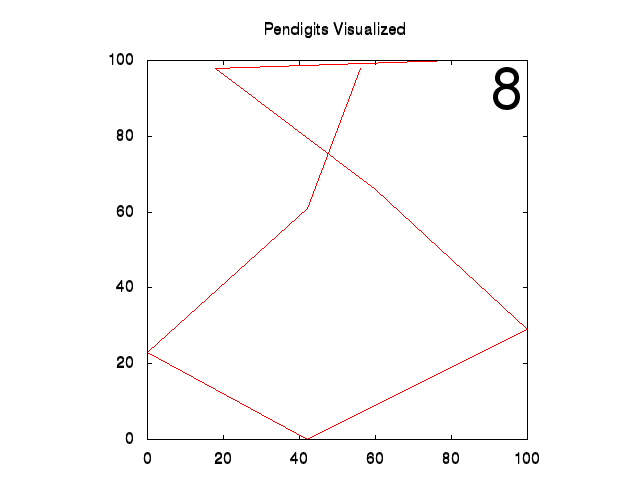
\includegraphics[scale=0.3,bb=0 0 640 480]{pendigit-testing1.png}
			    \caption{Testdaten}
			    \label{picture-label}
			 \end{figure}\\
			\begin{figure}[h!]
 			   \centering
			    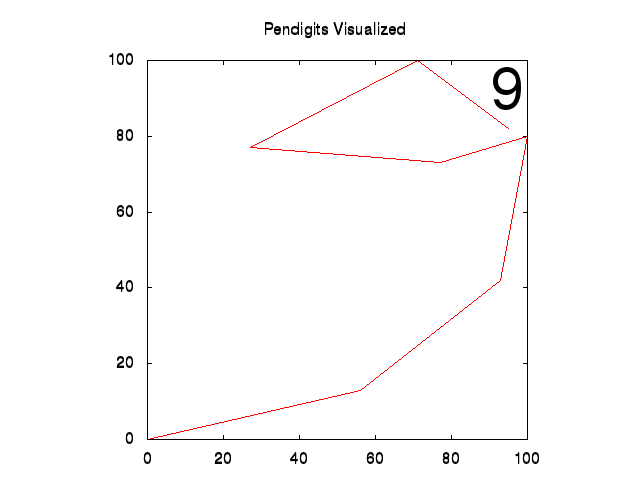
\includegraphics[scale=0.3,bb=0 0 640 480]{pendigit-testing3.png}
			    \caption{Testdaten}
			    \label{picture-label}
			 \end{figure}
		
		\subsection*{2. Source-Code}
			Code mit Kommentaren auf separatem Blatt
		
		\subsection*{3. Beschreibung}
			Es wurden 1-NN und k-NN implementiert.
			\subsubsection*{a) 1-NN Implementierung}
				\begin{enumerate}
				\item \textbf{Trainingsphase: Feature-Extraktion}\\
					Die Trainingsdaten werden in eine Matrix eingelesen, und die Features (siehe c) berechnet und in einer Matrix gespeichert.
					
					Für eine einfachere Berechnung der Features werden die Eingabedaten in eine dreidimensionale Matrix überführt, mit folgenden Dimensionen.\\
					1: Zeile, repräsentiert ein Objekt (Testdatum)\\
					2: Nummer der Punktes (von 1 bis 8)\\
					3: Koordinate (1 für x oder 2 für y)
					
				\item \textbf{Erkennung mittels Nearest Neighbor Search}\\
					Die zu erkennenden Testdaten werden ebenso eingelesen und ihre Features berechnet.
					Die Erkennung erfolg mittels der einfachsten Implementierung von Nearest Neighbor Search, dem Linear Nearest Neighbor Search. Dabei werden für ein zu erkennendes Objekt alle Abstände (im Feature-Raum!) zu allen Testdaten berechnet und das Minimum berechnet.
					%\footnote{siehe \url{http://en.wikipedia.org/wiki/Nearest_neighbor_search#Linear_search} }.
					
					Die euklidische Abstandsberechnung haben wir so optimiert, dass nicht die Wurzel gezogen wird. Das ist möglich weil es gilt $ \sqrt{a} < \sqrt{b} \Rightarrow a < b $ und somit ist die Berechnung des Minimums (bzw. von k Minima) korrekt.
					
					Eine von uns nicht implementierte Optimierung wäre ein Space-Partitioning Ansatz wie Kd-Bäume.
					
				\item \textbf{Auswertung}\\
					Als Metriken werden ausgegeben:\\
					1) Vergangene Zeit für einzelne Schritte\\
					3) Fehlerrate = $ \dfrac{Anzahl Fehler}{Anzahl Testdaten} $\\
					4) Analyse für jede Zahl, mit welchen Zahlen sieh häufig verwechselt wurden, und wie oft sie korrekt erkannt wurde.
				\end{enumerate}
				
			\subsubsection*{b) K-NN}
				
				k-NN unterscheidet sich nur in der Erkennungsphase von 1-NN.
				
				Die Abstände werden diesmal berechnet und in einer Matrix gespeichert.
				Anschließend müssen die k Nachbarn mit dem geringsten Abstand gefunden werden. Dafür sortieren wir die Liste und nehmen die ersten k Elemente.
				Dann wird nachgesehen, in welchem Klassen die Nachbarn liegen, und die häufigste Klasse übernommen.
				
			\subsubsection*{c) Wahl der Features}
				In einem ersten Ansatz haben wir vier Features extrahiert, später kamen naive 16 Features hinzu, die direkt auf den Daten basieren.
				\begin{enumerate}
					\item \textbf{Entfernung von Anfang bis Ende}: Verwendet den euklidischen Abstand
					\item \textbf{Länge des Schriftzugs}: Summe der euklidischen Abstände zwischen den Punkten.
					\item \textbf{Verhältnis von Abstand zu Länge Schriftzug}: Definiert als  $ \dfrac{Feature 1}{Feature 2} $
					\item \textbf{Kumulierter Winkel}: Zuerst werden die Vektoren in freie Vektoren umgewandelt, d.h. jeder Vektor wird neu berechnet als relativer Abstand zum vorherigen Vektor. Anschließend werden die Winkel zwischen den freien Vektoren berechnet und summiert.
					\item \textbf{Naive Features (16 Features auf Basis der Punkte):} Jede x und jede x-Koordinate kann als Feature interpretiert werden, woraus 16 Features resultieren.
				\end{enumerate}
				
			
		\subsection*{4. Analyse}
			\subsubsection*{a) Laufzeitanalyse}
				Die Laufzeit der Trainingsphase bei n Trainingsdaten ist $ O(n) $, unter der Annahme, dass die Berechnung der einzelnen Merkmale konstant ist (realistisch).\\
				
				Die Laufzeit der 1-NN Erkennung für ein Objekts bei n Testdaten ist ebenso $ O(n) $, da der Abstand zu jedem anderem Testdatum im Feature-Raum berechnet werden muss.\\
				
				Die Laufzeit der k-NN Erkennung für ein Objekt bei n Testdaten ist $ O(n + n\ log\ n) = O(n) $, da der Abstand zu jedem Testobjekt berechnet werden muss, anschließend das Ergebnis sortiert wird. Die weiteren Schritte sind (angenommen k ist klein) zu vernachlässigen.\\
				
				Die Laufzeit der Erkennung ist, neben der Fehlerrate, der zweite wesentliche Faktor für einen Erkennungs-Algorithmus. NN und k-NN haben hier aufgrund ihrer linearen Laufzeit ihren erheblichen Nachteil.\\
				
				\textbf{Parallelisierung}: Der Nearest-Neighbor-Search für ein konktretes Objekt ist schlecht parallelisierbar, da das Minimum berechnet wird. Perfekt parallelisierbar ist jedoch der die Erkennung für n Objekte, so dass bei 8 Kernen jeder Kern nur ein Achtel der Objekte erkennt. Das parfor Statement in Matlab ermöglicht diese Parallelisierung.
				
			
			\subsubsection*{b) Ergebnisse}
				Bemerkung: Das Feature 'Kummulierter Winkel' wurde bei der Analyse nicht berücksichtigt. Wir haben den Code ursprünglich für Octave geschrieben und konnten die Winkelberechnung nicht so schnell für Matlab umschreiben (wo unsere parallelisierte Auswertung lief). Die Ergebnisse für die drei Feature fallen seit dem wesentlich schlechter aus als die vorherigen Octave-Ergebnisse mit kumuliertem Winkel (damals 20\% Fehlerrate).\\
				
				Im folgenden eine Übersicht über die Fehlerrate in Abhängigkeit von k und den gewählten Features.
				\begin{table}[h!]
				    \begin{tabular}{|l|l|l|l|}
				        \hline
     					   ~  & 3 Features    & 16 naive Features   & Alle 19 Features \\ \hline
					        k=1  & 0.6   & 0.031 & 0.040 \\ 
					        k=3  & 0.578 & 0.026 & 0.037 \\ 
					        k=5  & 0.555 & 0.032 & 0.043 \\ 
					        k=15 & 0.539 & 0.038 & 0.053 \\
				        \hline
				    \end{tabular}
				\end{table}
				
				Die naiven Features ermöglichen mit Abstand die beste Klassifikation. Sie haben den Nachteil, dass die Dimension nicht verringert wurden.\\
				
				Die 3 Features bieten mit 20\% (mit kumuliertem Winkel) eine akzeptable Erkennungsrate. Diese kann noch verbessert werden, wenn die \textbf{Features normalisiert} werden. Aktuell ist es so, dass die Merkmale, die einen großen Wertebereich haben, stärker bei der Abstandsberechnung berücksichtigt werden, weshalb alle den gleichen Wertebereich haben sollten.\\
				
				Durch mehr Features kann man sicher bessere Erkennungsraten erreichen.\\
				
				Bei k-NN fehlt außerdem die \textbf{Gewichtung der Nachbarn}. Sehr nahe Nachbarn sollten stärker berücksichtigt werden als weit entfernte Nachbarn. Wikipedia schlägt (1/distance) als Gewicht vor.
				
		\subsection*{5. Beispielausgabe}
			Im folgenden eine Beispielausgabe für 3-NN.
		\begin{verbatim}

** TESTRUN **

training-rows: 4000
test-rows: 2000
use k-nn? 1
k: 3

Seconds Training Feature Extraction:  0.487561
Seconds Test Feature Extraction:  0.253212
Seconds Prediction:  70.845423
>> analyze
 
** RESULTS **

hits for 0: 211
hits for 1: 204
hits for 2: 203
hits for 3: 180
hits for 4: 199
hits for 5: 190
hits for 6: 194
hits for 7: 205
hits for 8: 196
hits for 9: 166
Number 0, missclassified as 6: 5
 Number 0, missclassified as 8: 1
Number 0, missclassified as 9: 1
Number 1, missclassified as 2: 7
Number 1, missclassified as 4: 1
Number 2, missclassified as 1: 1
Number 3, missclassified as 1: 1
Number 3, missclassified as 9: 1
 Number 4, missclassified as 5: 6
Number 5, missclassified as 3: 3
Number 7, missclassified as 1: 12
Number 7, missclassified as 2: 1
Number 8, missclassified as 0: 1
Number 8, missclassified as 5: 1
Number 9, missclassified as 1: 3
 Number 9, missclassified as 3: 2
Number 9, missclassified as 4: 1
Number 9, missclassified as 5: 2
Number 9, missclassified as 7: 2

Total classifications: 2000
Total hits: 1948
Total misses: 52
ERROR RATE: 0.026
		\end{verbatim}
		
		
\end{document}
